\documentclass[11pt,a4paper]{article}

\usepackage[utf8]{inputenc}
\usepackage[T1]{fontenc}
\usepackage{mathpazo}
\usepackage[scaled=0.92]{helvet}
\usepackage[margin=1in]{geometry}
\usepackage{graphicx}
\usepackage{amsmath,amssymb,amsfonts}
\usepackage{booktabs}
\usepackage{tabularx}
\usepackage{setspace}
\usepackage{titlesec}
\usepackage{fancyhdr}
\usepackage{float}
\usepackage{caption}
\usepackage{microtype}
\usepackage{tikz}
\usepackage{xcolor}
\usepackage[hidelinks]{hyperref}

\usetikzlibrary{shapes.geometric, arrows.meta, positioning, calc, matrix, fit, backgrounds}

\setstretch{1.15}
\setlength{\parindent}{0pt}
\setlength{\parskip}{0.8em}
\sloppy

\titleformat{\section}{\normalfont\large\bfseries\sffamily}{\thesection}{1em}{}
\titleformat{\subsection}{\normalfont\normalsize\bfseries\sffamily}{\thesubsection}{1em}{}
\titleformat{\subsubsection}{\normalfont\normalsize\itshape\sffamily}{\thesubsubsection}{1em}{}

\pagestyle{fancy}
\fancyhf{}
\fancyhead[L]{\small\sffamily Panduan Format Referensi LaTeX}
\fancyhead[R]{\small\sffamily\thepage}
\renewcommand{\headrulewidth}{0.4pt}

\captionsetup{font=small,labelfont=bf,labelsep=period}

\renewenvironment{abstract}
{\small
	\begin{center}\textbf{\sffamily Abstrak}\end{center}
	\begin{quote}}
	{\end{quote}}

\lstdefinestyle{code}{
	basicstyle=\ttfamily\small,
	frame=single,
	rulecolor=\color{black},
	breaklines=true,
	showstringspaces=false,
	columns=fullflexible,
	keepspaces=true,
	framesep=6pt,
	aboveskip=1em,
	belowskip=1em,
	xleftmargin=0pt
}

\lstdefinestyle{out}{
	basicstyle=\ttfamily\small,
	frame=tb,
	rulecolor=\color{black},
	breaklines=true,
	showstringspaces=false,
	columns=fullflexible,
	keepspaces=true,
	framesep=4pt,
	aboveskip=1em,
	belowskip=1em
}

\title{\vspace{-1.5cm}\textbf{\sffamily\LARGE Panduan Format Referensi dalam LaTeX\\ Dua Belas Tipe Sumber Akademik}}
\author{
	\textbf{Muhammad Riduwan Khafidi} \\
	\small Program Studi Teknik Rekayasa Perangkat Lunak \\
	\small Politeknik Negeri Batam \\
	\small \texttt{4342611034@students.polibatam.ac.id}
}
\date{\small\today}

\begin{document}

\maketitle
\thispagestyle{empty}

\begin{abstract}
	Daftar pustaka sering menjadi bagian yang paling terabaikan dalam penulisan makalah akademik, padahal ia adalah jejak integritas seorang penulis. Makalah ini menyajikan dua belas pola format referensi yang lazim muncul di makalah teknik dan ilmu komputer, mulai dari buku teks, artikel jurnal, prosiding konferensi, RFC, standar teknis, hingga dokumentasi resmi dan artikel website. Setiap pola disertai contoh konkret yang bisa disalin langsung ke dalam berkas \texttt{.tex}, serta penjelasan singkat kapan pola tersebut dipakai. Pembaca akan memperoleh kerangka yang jelas untuk menyusun daftar pustaka yang konsisten di seluruh seri makalahnya.
\end{abstract}

\section{Pendahuluan}

Daftar pustaka bukan sekadar lampiran. Ia adalah kontrak antara penulis dan pembaca: bahwa setiap klaim yang diajukan dapat ditelusuri kembali ke sumber aslinya. Dalam LaTeX, kontrak itu diwujudkan lewat pasangan \texttt{\textbackslash cite} di badan teks dan \texttt{\textbackslash bibitem} di daftar pustaka.

Makalah ini menyajikan dua belas pola referensi yang paling sering dipakai. Setiap pola ditulis dalam bentuk blok \texttt{bibitem} yang siap disalin, disertai contoh konkret. Semua contoh mengikuti gaya yang sama: nama belakang penulis, tahun dalam tanda kurung, judul dalam italic, penerbit atau URL.

\section{Anatomi Satu Entri Referensi}

Sebelum masuk ke dua belas pola, mari perhatikan anatomi satu entri pada Gambar~\ref{fig:anatomy-ref}.

\begin{figure}[H]
	\centering
	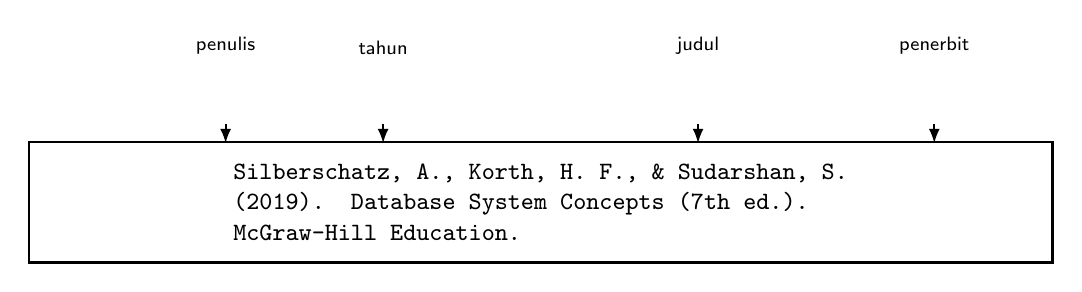
\begin{tikzpicture}[
			box/.style={rectangle, draw=black, thick, minimum width=13cm, minimum height=1.5cm, align=left, font=\ttfamily\small, inner sep=8pt},
			label/.style={font=\sffamily\small}
		]
		\node[box, fill=white] (entry) at (0, 0) {
			Silberschatz, A., Korth, H. F., \& Sudarshan, S. \\
			(2019). Database System Concepts (7th ed.). \\
			McGraw-Hill Education.
		};

		\draw[thick, -latex] (-4, 1.0) -- (-4, 0.75) node[above=1cm, font=\scriptsize\sffamily] {penulis};
		\draw[thick, -latex] (-2, 1.0) -- (-2, 0.75) node[above=1cm, font=\scriptsize\sffamily] {tahun};
		\draw[thick, -latex] (2, 1.0) -- (2, 0.75) node[above=1cm, font=\scriptsize\sffamily] {judul};
		\draw[thick, -latex] (5, 1.0) -- (5, 0.75) node[above=1cm, font=\scriptsize\sffamily] {penerbit};
	\end{tikzpicture}
	\caption{Anatomi satu entri referensi.}
	\label{fig:anatomy-ref}
\end{figure}

Lima bagian wajib dalam satu entri: nama penulis, tahun, judul, penerbit, dan (untuk sumber daring) URL. Urutannya tidak berubah antar tipe sumber.

\section{Dua Belas Pola Referensi}

\subsection{Pola 1: Buku Teks}

Dipakai untuk buku cetak yang menjadi rujukan utama.

\begin{lstlisting}[style=code]
\bibitem{silberschatz}
Silberschatz, A., Korth, H. F., \& Sudarshan, S. (2019).
\textit{Database System Concepts} (7th ed.).
McGraw-Hill Education.
\end{lstlisting}

Perhatikan tiga hal. Pertama, nama depan disingkat untuk penulis kedua ke atas. Kedua, edisi ditulis dalam tanda kurung biasa setelah judul. Ketiga, judul dalam \texttt{\textbackslash textit\{\}}.

\subsection{Pola 2: Buku Terjemahan}

\begin{lstlisting}[style=code]
\bibitem{sommerville}
Sommerville, I. (2016).
\textit{Software Engineering} (10th ed.).
Pearson.
\end{lstlisting}

\subsection{Pola 3: Bab dalam Buku yang Disunting}

\begin{lstlisting}[style=code]
\bibitem{kleppmann-chapter}
Kleppmann, M. (2017).
Encoding and Evolution.
In \textit{Designing Data-Intensive Applications}
(pp. 111--146).
O'Reilly Media.
\end{lstlisting}

\subsection{Pola 4: Artikel Jurnal}

\begin{lstlisting}[style=code]
\bibitem{stonebraker}
Stonebraker, M., \& Cattell, R. (2011).
Ten Rules for Scalable Performance in Simple
Operation Datastores.
\textit{Communications of the ACM}, 54(6), 72--80.
\texttt{https://doi.org/10.1145/1953122.1953144}
\end{lstlisting}

Nomor volume, edisi, dan halaman wajib dicantumkan. DOI ditulis dengan awalan URL lengkap.

\subsection{Pola 5: Prosiding Konferensi}

\begin{lstlisting}[style=code]
\bibitem{chandra}
Chandra, T., \& others. (2019).
Ray: A Distributed Framework for Emerging AI
Applications.
In \textit{Proceedings of the 13th USENIX Symposium
on Operating Systems Design and Implementation}
(pp. 561--577). USENIX Association.
\end{lstlisting}

\subsection{Pola 6: Tesis dan Disertasi}

\begin{lstlisting}[style=code]
\bibitem{tesis}
Pratama, A. (2023).
\textit{Optimasi Query Basis Data Relasional
pada Sistem Terdistribusi}.
Tesis magister, Politeknik Negeri Batam.
\end{lstlisting}

Untuk skripsi, gunakan kata "skripsi". Untuk disertasi doktoral, gunakan "disertasi". Untuk tesis magister, gunakan "tesis".

\subsection{Pola 7: RFC IETF}

\begin{lstlisting}[style=code]
\bibitem{rfc4122}
Leach, P., Mealling, M., \& Salz, R. (2005).
\textit{A Universally Unique IDentifier (UUID)
URN Namespace} (RFC 4122). IETF.
\end{lstlisting}

Nomor RFC ditulis dalam tanda kurung setelah judul. Penerbitnya selalu IETF.

\subsection{Pola 8: Standar Teknis}

\begin{lstlisting}[style=code]
\bibitem{ieee754}
IEEE. (2019).
\textit{IEEE Standard for Floating-Point Arithmetic
(IEEE 754-2019)}.
Institute of Electrical and Electronics Engineers.
\end{lstlisting}

Untuk standar W3C, ISO, atau ANSI, polanya sama. Nama organisasi sebagai penulis, tahun, judul lengkap termasuk nomor standar, lalu nama organisasi lengkap sebagai penerbit.

\subsection{Pola 9: Dokumentasi Resmi}

\begin{lstlisting}[style=code]
\bibitem{mariadb-ddl}
MariaDB Foundation. (2026).
\textit{SQL Statements --- CREATE TABLE, ALTER TABLE,
DROP TABLE}.
MariaDB Knowledge Base.
\texttt{https://mariadb.com/kb/en/sql-statements/}
\end{lstlisting}

Dokumentasi resmi memakai nama proyek atau organisasi sebagai penulis. Tanggal akses sering tidak dicantumkan karena dokumentasi biasanya diperbarui.

\subsection{Pola 10: Artikel Website}

\begin{lstlisting}[style=code]
\bibitem{mozilla-mdn}
Mozilla. (2026).
\textit{CSS Grid Layout}.
MDN Web Docs.
\texttt{https://developer.mozilla.org/en-US/docs/Web/CSS/CSS_grid_layout}
\end{lstlisting}

\subsection{Pola 11: Entri Ensiklopedia}

\begin{lstlisting}[style=code]
\bibitem{sobolev}
Sobolev, S. K. (n.d.).
Individual variable.
In \textit{Encyclopedia of Mathematics}.
Springer.
\texttt{http://encyclopediaofmath.org/index.php?title=Individual\_variable}
\end{lstlisting}

\texttt{n.d.} adalah singkatan dari \textit{no date}, dipakai ketika tahun terbit tidak tersedia.

\subsection{Pola 12: Wikipedia dan Sumber Berubah}

\begin{lstlisting}[style=code]
\bibitem{wikipedia-cs}
Wikipedia Contributors. (2026, October 30).
\textit{Variable (high-level programming language)}.
Wikipedia, The Free Encyclopedia.
\texttt{https://en.wikipedia.org/wiki/Variable\_(high-level\_programming\_language)}
\end{lstlisting}

Wikipedia jarang diterima sebagai sumber utama di makalah akademik. Jika harus dipakai, cantumkan tanggal lengkap versi artikel yang diakses, karena artikel Wikipedia bisa berubah kapan saja.

\section{Tabel Perbandingan Format}

\begin{table}[H]
	\centering
	\caption{Perbandingan format antar tipe referensi.}
	\label{tab:ref-types}
	\footnotesize
	\begin{tabularx}{\textwidth}{l X X}
		\toprule
		Tipe         & Unsur Khas                     & Kapan Dipakai                    \\
		\midrule
		Buku teks    & edisi dalam kurung             & rujukan utama, konsep dasar      \\
		Bab buku     & halaman dan editor             & bab spesifik yang relevan        \\
		Jurnal       & volume, edisi, halaman, DOI    & penelitian terkini               \\
		Konferensi   & nama prosiding, halaman        & temuan awal, riset baru          \\
		Tesis        & jenis tesis dan institusi      & karya lokal, arsip kampus        \\
		RFC          & nomor RFC                      & protokol internet                \\
		Standar      & nomor standar, organisasi      & spesifikasi teknis resmi         \\
		Dokumentasi  & URL resmi proyek               & referensi teknis perangkat lunak \\
		Website      & URL dan penerbit               & sumber sekunder                  \\
		Ensiklopedia & \texttt{n.d.} jika tanpa tahun & definisi singkat                 \\
		Wikipedia    & tanggal lengkap                & hanya jika terpaksa              \\
		\bottomrule
	\end{tabularx}
\end{table}

\section{Contoh Daftar Pustaka Lengkap}

Berikut contoh daftar pustaka yang menggabungkan dua belas pola di atas. Contoh ini bisa disalin langsung ke dalam berkas \texttt{.tex} baru.

\begin{lstlisting}[style=code]
\newpage
\section*{Referensi}
\addcontentsline{toc}{section}{Referensi}

\begin{thebibliography}{99}

	\bibitem{babbie}
	Babbie, E. R. (2009).
	\textit{The Practice of Social Research} (12th ed.).
	Wadsworth Publishing.

	\bibitem{boyer}
	Boyer, C. B. (1991).
	\textit{A History of Mathematics}.
	John Wiley \& Sons.

	\bibitem{brookshear}
	Brookshear, J. G. (2019).
	\textit{Computer Science: An Overview} (13th ed.).
	Pearson.

	\bibitem{chandra}
	Chandra, T., \& others. (2019).
	Ray: A Distributed Framework for Emerging AI Applications.
	In \textit{Proceedings of the 13th USENIX Symposium on
	Operating Systems Design and Implementation}
	(pp. 561--577). USENIX Association.

	\bibitem{ieee754}
	IEEE. (2019).
	\textit{IEEE Standard for Floating-Point Arithmetic
	(IEEE 754-2019)}.
	Institute of Electrical and Electronics Engineers.

	\bibitem{klabnik}
	Klabnik, S., \& Nichols, C. (2019).
	\textit{The Rust Programming Language}.
	No Starch Press.

	\bibitem{kleppmann}
	Kleppmann, M. (2017).
	\textit{Designing Data-Intensive Applications}.
	O'Reilly Media.

	\bibitem{mariadb-ddl}
	MariaDB Foundation. (2026).
	\textit{SQL Statements --- CREATE TABLE, ALTER TABLE,
	DROP TABLE}.
	MariaDB Knowledge Base.
	\texttt{https://mariadb.com/kb/en/sql-statements/}

	\bibitem{mysql-ddl}
	Oracle Corporation. (2026).
	\textit{MySQL 8.0 Reference Manual --- Data Definition
	Statements}.
	\texttt{https://dev.mysql.com/doc/refman/8.0/en/sql-data-definition-statements.html}

	\bibitem{postgresql}
	The PostgreSQL Global Development Group. (2026).
	\textit{Chapter 8. Data Types}.
	PostgreSQL Documentation.
	\texttt{https://www.postgresql.org/docs/current/datatype.html}

	\bibitem{rfc4122}
	Leach, P., Mealling, M., \& Salz, R. (2005).
	\textit{A Universally Unique IDentifier (UUID)
	URN Namespace} (RFC 4122). IETF.

	\bibitem{silberschatz}
	Silberschatz, A., Korth, H. F., \& Sudarshan, S. (2019).
	\textit{Database System Concepts} (7th ed.).
	McGraw-Hill Education.

	\bibitem{stonebraker}
	Stonebraker, M., \& Cattell, R. (2011).
	Ten Rules for Scalable Performance in Simple Operation
	Datastores.
	\textit{Communications of the ACM}, 54(6), 72--80.
	\texttt{https://doi.org/10.1145/1953122.1953144}

	\bibitem{zig}
	Zig Software Foundation. (2026).
	\textit{Language Reference --- Primitive Types}.
	\texttt{https://ziglang.org/documentation/master/}

\end{thebibliography}
\end{lstlisting}

\section{Kesalahan Umum pada Daftar Pustaka}

\begin{table}[H]
	\centering
	\caption{Kesalahan umum pada daftar pustaka.}
	\label{tab:ref-mistakes}
	\footnotesize
	\begin{tabularx}{\textwidth}{l X X}
		\toprule
		Kesalahan                                                          & Akibat                & Perbaikan                                                                        \\
		\midrule
		\texttt{\textbackslash cite} tanpa \texttt{\textbackslash bibitem} & muncul tanda tanya    & lengkapi \texttt{bibitem}                                                        \\
		\texttt{\textbackslash bibitem} tanpa \texttt{\textbackslash cite} & entri tidak muncul    & tambahkan \texttt{\textbackslash cite} atau pakai \texttt{\textbackslash nocite} \\
		judul tanpa italic                                                 & gaya tidak konsisten  & pakai \texttt{\textbackslash textit}                                             \\
		URL tanpa \texttt{\textbackslash texttt}                           & URL tidak terbaca     & bungkus dalam \texttt{\textbackslash texttt}                                     \\
		ampersand tanpa escape                                             & error kompilasi       & tulis \texttt{\textbackslash\&}                                                  \\
		tahun tanpa kurung                                                 & gaya tidak konsisten  & tulis \texttt{(tahun)}                                                           \\
		nama depan panjang                                                 & memakan ruang         & singkat jadi inisial                                                             \\
		kunci \texttt{bibitem} duplikat                                    & rujukan salah sasaran & pastikan kunci unik                                                              \\
		\bottomrule
	\end{tabularx}
\end{table}

\section{Kesimpulan}

Tiga prinsip penutup untuk daftar pustaka yang konsisten:

\begin{enumerate}
	\item Pilih satu gaya dan patuhi. Jangan campur gaya APA dengan gaya IEEE dalam satu makalah. Pilih satu, terapkan ke semua entri.
	\item Setiap klaim punya jejak. Jika dalam badan teks tertulis "menurut penelitian X", maka harus ada \texttt{\textbackslash cite} ke entri X di daftar pustaka.
	\item Kualitas sumber menentukan kualitas makalah. Dokumentasi resmi dan buku teks lebih kuat daripada artikel blog. Wikipedia hanya dipakai jika benar-benar tidak ada sumber primer.
\end{enumerate}

Dengan dua belas pola ini, seluruh kebutuhan referensi makalah teknik dan ilmu komputer dapat dipenuhi tanpa perlu menghafal gaya baru.

\newpage
\section*{Referensi}
\addcontentsline{toc}{section}{Referensi}

\begin{thebibliography}{99}

	\bibitem{lamport}
	Lamport, L. (1994).
	\textit{LaTeX: A Document Preparation System} (2nd ed.).
	Addison-Wesley.

	\bibitem{mittelbach}
	Mittelbach, F., \& Goossens, M. (2004).
	\textit{The LaTeX Companion} (2nd ed.).
	Addison-Wesley.

	\bibitem{ieee754}
	IEEE. (2019).
	\textit{IEEE Standard for Floating-Point Arithmetic
		(IEEE 754-2019)}.
	Institute of Electrical and Electronics Engineers.

	\bibitem{rfc4122}
	Leach, P., Mealling, M., \& Salz, R. (2005).
	\textit{A Universally Unique IDentifier (UUID)
		URN Namespace} (RFC 4122). IETF.

	\bibitem{mariadb-ddl}
	MariaDB Foundation. (2026).
	\textit{SQL Statements --- CREATE TABLE, ALTER TABLE,
		DROP TABLE}.
	MariaDB Knowledge Base.
	\texttt{https://mariadb.com/kb/en/sql-statements/}

	\bibitem{silberschatz}
	Silberschatz, A., Korth, H. F., \& Sudarshan, S. (2019).
	\textit{Database System Concepts} (7th ed.).
	McGraw-Hill Education.

\end{thebibliography}

\end{document}
